%% CS-E4780 course project report: Detecting Trading Trends in Financial Tick Data
%% Built on the official ACM sigconf template (acmart).
%%
%% How to use this file:
%%   1. Upload report.tex, references.bib and the figures/ folder to one Overleaf project
%%      (or run `latexmk -pdf report.tex` inside report/).
%%   2. Search for "TODO". Red \todo{} markers show in the PDF; each one points at a
%%      "FACT SHEET" comment block just above it. Those blocks list what we measured, the
%%      possible explanations and the numbers behind each one. Write the paragraph in your
%%      own words, then delete the fact sheet and the marker.
%%   3. Delete every helper comment before you submit.
%%   4. Keep the whole thing at 4-5 pages. Don't touch margins, fonts or spacing.
%%
%% Who wrote what (keep this honest for the AI-use note):
%%   - Your own text from the draft is kept as it was, except where a fact was wrong.
%%     Every such fix is marked with a "%% FIXED:" comment saying what changed and why.
%%   - The setup, method, result numbers, tables, figure captions and the architecture
%%     figure were written with Claude from the repository's results/ folder.
%%   - The analysis, interpretation, conclusions and contribution text are left for you.

\documentclass[sigconf]{acmart}
\usepackage{tikz}
\usetikzlibrary{positioning,fit,arrows.meta}
\graphicspath{{figures/}}

%% The template loads xcolor already, so this little marker is safe to use.
%% It just prints a red reminder in the PDF so nothing half-finished slips through.
\newcommand{\todo}[1]{\textcolor{red}{[TODO: #1]}}

%% Placeholder conference info. The course example report keeps the default
%% ACM reference-format block and copyright footer, so we do the same.
\acmConference[CS-E4780]{CS-E4780 Scalable Systems and Data Management}{Autumn 2026}{Espoo, Finland}

\begin{document}

\title{Detecting Trading Trends in Financial Tick Data}
\subtitle{\small CS-E4780 Scalable Systems and Data Management Course Project}

%% One \author block per person. Use full first names, no initials.
\author{Yashasvi Mishra}
\affiliation{%
  \institution{Aalto University}
  \city{Espoo}
  \country{Finland}}
  \email{yashasvi.mishra@aalto.fi}

\author{Manas Vernekar}
\affiliation{%
  \institution{Aalto University}
  \city{Espoo}
  \country{Finland}}
  \email{manas.vernekar@aalto.fi}

\renewcommand{\shortauthors}{{Mishra} and {Vernekar}}

%% ---------------------------------------------------------------------------
\begin{abstract}
%% FIXED: the validation was not against "a reference dataset provided for the course"
%% but against our own pandas answer key for the whole working week (1,855,645 windows).
%% The rest is your text unchanged.
This project implements a real-time financial tick data processing system using Apache Kafka and Apache Flink. Incoming trade events are streamed through Kafka, processed using event-time tumbling windows, and analysed with Exponential Moving Average (EMA) indicators. Two EMAs, EMA38 and EMA100, are calculated for each financial instrument to identify bullish and bearish market trends. The system generates buy and sell signals based on EMA crossovers and publishes the results to output Kafka topics. A Streamlit dashboard was developed to visualize processed results, trading signals, and EMA trends. The output for the full working week of the DEBS 2022 data was checked against an independent reference implementation and matched it in every one of its 1,855,645 windows and 11,349 advisories.
\todo{optional: add one sentence with your headline performance result, e.g.\ the 1 to 8 core throughput and the latency figure you find most important}
\end{abstract}

%% CCS concepts are required by the template once a paper is longer than two
%% pages. Generate the block at https://dl.acm.org/ccs (search for "stream" or
%% "distributed", pick 2-3 concepts, click "Generate CCS Code") and paste the
%% \begin{CCSXML} ... \end{CCSXML} plus the \ccsdesc lines right here.
%% Until you do, LaTeX prints a harmless warning. Don't invent the IDs by hand.

%% FIXED: removed the empty item (double comma) from the keyword list.
\keywords{Apache Flink, Apache Kafka, stream processing, complex event processing, exponential moving average, tick data}

\maketitle

%% ---------------------------------------------------------------------------
\section{Introduction}
%% FIXED: "a Kafka output topic" -> "Kafka output topics" (results, advisories and late
%% trades go to three topics). Added the dataset citation. Otherwise your text.
Modern financial markets generate large volumes of real-time trading data that must be processed with low latency. Traditional batch processing approaches are insufficient for detecting market trends and trading opportunities as events arrive continuously throughout the trading day. The objective of this project was to build a scalable stream-processing system capable of analysing financial tick data in real time, using the DEBS 2022 Grand Challenge data set~\cite{frischbier2022gc,frischbier2022debs}. The project uses Apache Kafka~\cite{kreps2011kafka} for event ingestion and Apache Flink~\cite{carbone2015flink} for distributed stream processing. Financial events are grouped into five-minute tumbling event-time windows and used to calculate Exponential Moving Averages (EMA38 and EMA100) for each financial instrument. Two analytical queries were implemented. The first query computes EMA values for each financial instrument, while the second query detects bullish and bearish market breakouts based on EMA crossover events. Results are published to Kafka output topics and visualized through an interactive Streamlit dashboard. The implementation demonstrates the use of event-time processing, stateful stream computation, real-time analytics and dashboard visualization within a modern data-streaming architecture.
The source code and reproducibility instructions are available in the project's public GitHub repository: \url{https://github.com/The5pecial0ne/ssdm-financial-tick-data}.

%% ---------------------------------------------------------------------------
\section{Dataset Analysis}\label{sec:data}
%% The rubric asks for a "strong focus on dataset analysis" and for "handling of long-tail
%% distributions". The numbers below are facts from the data; the paragraph is yours.

The data set~\cite{frischbier2022debs} covers one week (Monday 8 to Sunday 14 November 2021) of tick data from three exchanges: Paris (FR), Amsterdam (NL) and Frankfurt (ETR). Table~\ref{tab:data} summarises it and Figure~\ref{fig:longtail} shows how the events spread over the symbols.

\begin{table}[t]
  \caption{The DEBS 2022 data, whole week, every event type. Trades are events with a price ($\mathit{Last}>0$); only they enter the windows.}
  \label{tab:data}
  \small
  \begin{tabular}{lrr}
    \toprule
    & Events & Symbols\\
    \midrule
    Paris (FR)       & 158,331,078 & 2,540\\
    Amsterdam (NL)   &  79,991,190 &   750\\
    Frankfurt (ETR)  &  50,794,540 & 2,212\\
    \midrule
    All exchanges    & 289,116,808 & 5,502\\
    Trades, Mon--Fri &  59,391,670 & 4,970\\
    5-minute windows with a trade, Mon--Fri & 1,855,645 & 4,970\\
    \bottomrule
  \end{tabular}
\end{table}

\begin{figure*}[t]
  \centering
  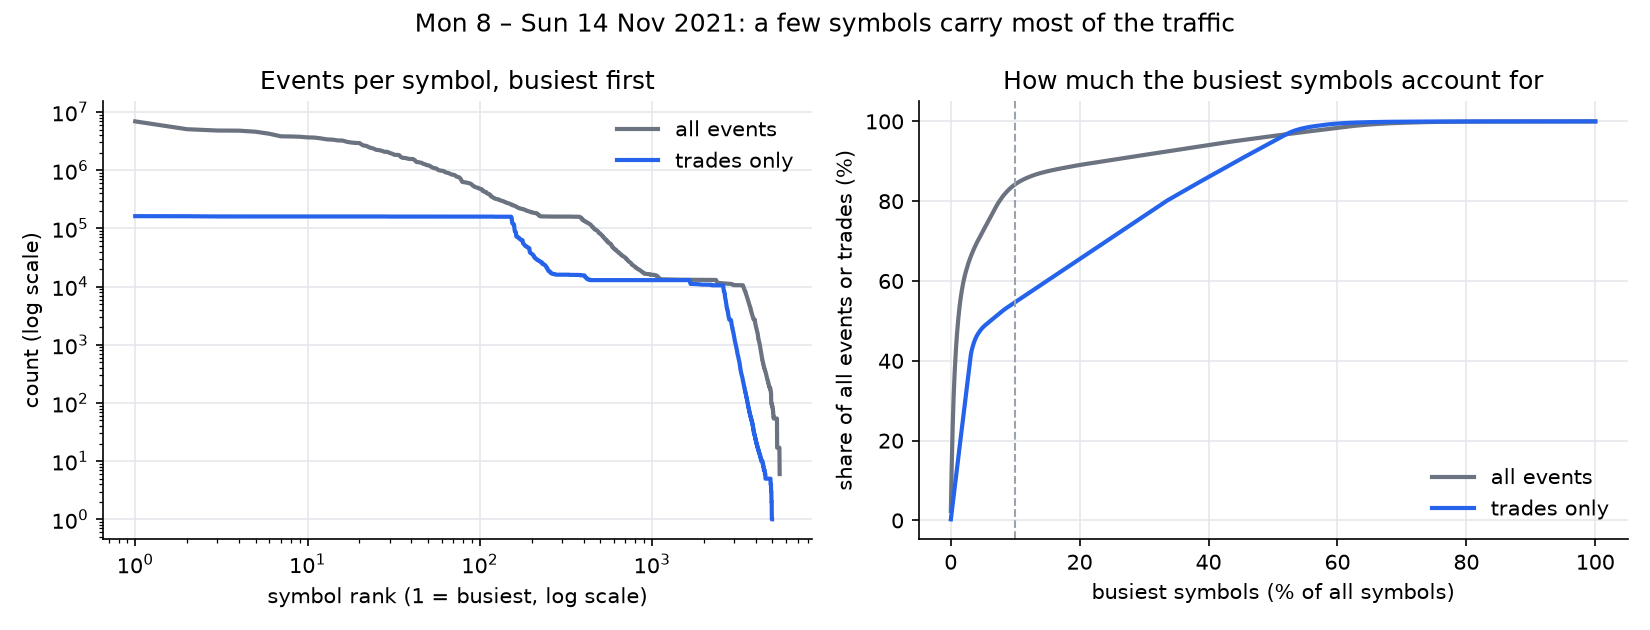
\includegraphics[width=0.85\linewidth]{longtail-week}
  \caption{Long tail of the symbol distribution over the whole week. Left: events per symbol, busiest first (log-log). Right: share of all events or trades covered by the busiest symbols; the dashed line marks the top 10\%. Produced by \texttt{analysis/longtail.py}.}
  \Description{Two line charts. The left one shows event counts per symbol falling steeply over five orders of magnitude, with trades flatter than all events. The right one shows the top 10 percent of symbols covering about 84 percent of all events but only about half of the trades.}
  \label{fig:longtail}
\end{figure*}

%% FACT SHEET: dataset analysis (write 1-2 paragraphs from this)
%% What we observed (all numbers checked against the data on 24 Nov):
%%  - 289.1 M events over 5,502 symbols for the week. Paris has the most events
%%    (158.3 M, 55%), Amsterdam has few symbols (750) but 80.0 M events, so the most
%%    events per symbol.
%%  - Long tail, all events: the top 1% of symbols carry 47.3% of all events, the top
%%    10% carry 84.2%; just 63 symbols make up half of everything. The busiest symbol is
%%    RDSA.NL with 6.9 M events; the median symbol has 11,225.
%%  - Trades are only about a fifth of the events (59.4 M trades Mon-Fri). The rest are
%%    quotes and housekeeping events with no price; the job counts and drops them.
%%  - Trades are much LESS skewed than events (right panel: top 10% of symbols is only
%%    about half of the trades). In the left panel the trade curve is flat at roughly
%%    1.6e5 trades for the top ~150 symbols. On Monday the busiest symbols have about 32k
%%    trades each (A0X7J3.ETR 32,371) and the median symbol 2,102.
%%  - On Monday, 9.81 M of the 11.79 M trades (83%) are on indices (SecType I) and 1.98 M
%%    on equities (E).
%%  - Windows per symbol over the week: median 530, but 1,605 of the 4,970 symbols have
%%    fewer than 100 windows and 1,263 have fewer than 38. For those, EMA100 (and often
%%    EMA38) never gets past the warm-up from EMA_0 = 0, so their advisories say more
%%    about the warm-up than about a real trend.
%%  - Saturday and Sunday contain events but almost no trades (the prices files for 13
%%    and 14 Nov are nearly empty), so the experiments use Mon-Fri.
%%  - Monday has no out-of-order trades at all within a symbol (0 trades older than one
%%    already seen) and no placeholder trading times. Earlier exploration
%%    (analysis/late_check.py) found trades stamped 01:00:00.000 on some other days;
%%    the job treats that exact time as a placeholder and drops it. Re-run
%%    late_check.py on your Mac if you want the exact per-day counts in the text.
%%  - The two clocks: on Monday 861 trades have a receive time ("Time") more than 60 s
%%    away from their trading time; "Time" is only precise to whole seconds (99.99% end
%%    in .000). That is why we use "Trading time" as event time.
%% Points worth making (your call which, and your interpretation):
%%  - What the long tail means for partitioning: keyBy(symbol) spreads ~5,000 keys over
%%    the parallel instances, and since no single symbol is more than ~2.4% of events,
%%    no single key can overload one instance (Section 5.5 measures this).
%%  - Why filtering quotes early matters for throughput (they are 80% of the input).
%%  - The warm-up artefact for rare symbols, and how the dashboard deals with it.
\todo{dataset analysis paragraph, see the fact sheet in the source}

%% ---------------------------------------------------------------------------
\section{System Architecture}\label{sec:arch}

\subsection{Overview}
%% FIXED: the input topic is called "ticks" (not "trading-events"), it has 8 partitions
%% keyed by symbol, and the job writes three topics, not one.
The implemented system follows an event-driven architecture built around Apache Kafka and Apache Flink (Figure~\ref{fig:architecture}). Historical financial tick data is replayed through a Python Kafka producer and published to the \texttt{ticks} topic, which has eight partitions and uses the symbol as message key, so all events of one symbol stay in order in one partition. Apache Flink consumes the incoming stream, assigns event-time timestamps and watermarks, performs windowed aggregations and computes Exponential Moving Averages (EMA38 and EMA100) for each traded symbol. The resulting EMA values are published to the Kafka topic \texttt{ema-results}, the buy and sell advisories additionally to \texttt{advisories}, and trades that arrive too late for their window to \texttt{late-trades}. A Streamlit-based dashboard consumes the processed results and visualizes trading signals, EMA trends and summary statistics. The architecture separates event production, stream processing and visualization, allowing each component to evolve independently.

%% FIXED: replaced the old flowchart image. It showed the October prototype (topic
%% "trading-events", test-slice.csv as the only input, no partitions, one output topic),
%% and its file name had spaces, which breaks \includegraphics. This one is drawn in TikZ,
%% so there is no image file to upload.
\begin{figure}[t]
  \centering
  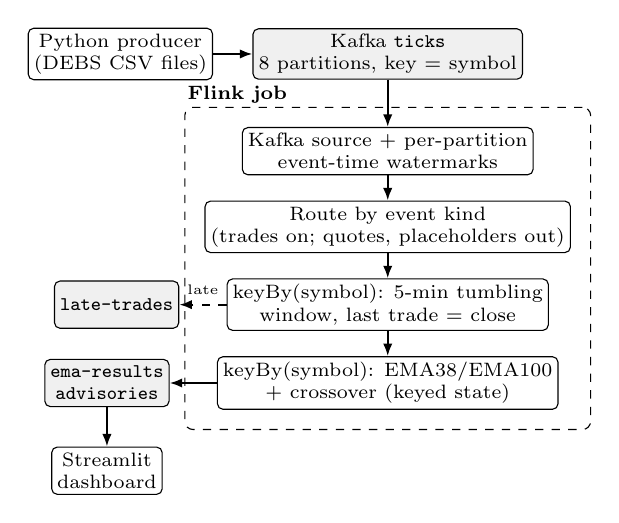
\begin{tikzpicture}[
      font=\scriptsize, node distance=3.2mm,
      box/.style={draw, rounded corners=2pt, align=center, minimum height=6mm, inner sep=2pt, fill=white},
      topic/.style={box, fill=black!6},
      op/.style={box, minimum width=31mm},
      arr/.style={-{Latex[length=1.6mm]}, thick}]
    \node[box] (prod) {Python producer\\(DEBS CSV files)};
    \node[topic, right=5mm of prod] (ticks) {Kafka \texttt{ticks}\\8 partitions, key = symbol};
    \node[op, below=6mm of ticks] (src) {Kafka source + per-partition\\event-time watermarks};
    \node[op, below=of src] (route) {Route by event kind\\(trades on; quotes, placeholders out)};
    \node[op, below=of route] (win) {keyBy(symbol): 5-min tumbling\\window, last trade = close};
    \node[op, below=of win] (ema) {keyBy(symbol): EMA38/EMA100\\+ crossover (keyed state)};
    \node[draw, dashed, rounded corners=3pt, inner sep=2.5mm, fit=(src)(route)(win)(ema),
          label={[font=\scriptsize\bfseries, anchor=south west, inner sep=1pt]north west:Flink job}] (flink) {};
    \node[topic, left=6mm of ema] (res) {\texttt{ema-results}\\\texttt{advisories}};
    \node[topic, left=6mm of win] (late) {\texttt{late-trades}};
    \node[box, below=5mm of res] (dash) {Streamlit\\dashboard};
    \draw[arr] (prod) -- (ticks);
    \draw[arr] (ticks) -- (src);
    \draw[arr] (src) -- (route);
    \draw[arr] (route) -- (win);
    \draw[arr] (win) -- (ema);
    \draw[arr] (ema) -- (res);
    \draw[arr, dashed] (win) -- node[above, font=\tiny]{late} (late);
    \draw[arr] (res) -- (dash);
  \end{tikzpicture}
  \caption{Pipeline. The producer replays the tick data into Kafka; the Flink job keeps only trades, closes 5-minute windows per symbol, updates both EMAs and emits an advisory on every crossover. Late trades go to a side output instead of being dropped silently.}
  \Description{Block diagram: a Python producer writes to the Kafka topic ticks. A Flink job with four stages (source with watermarks, routing by event kind, 5-minute window per symbol, EMA and crossover per symbol) reads it and writes to the topics ema-results and advisories, which feed a Streamlit dashboard, and to late-trades.}
  \label{fig:architecture}
\end{figure}

\subsection{Key design decisions}
%% FIXED: the watermark bullet now says where watermarks are made (per Kafka partition)
%% and that late trades are kept, which is what the code does. The rest is your text.
Several design decisions were made during implementation to improve correctness, modularity and maintainability.
\begin{itemize}
  \item Event-time processing was selected instead of processing-time processing because financial events naturally contain timestamps and may arrive out of order. Watermarks are generated per Kafka partition inside the source, with a bounded out-of-order allowance (5\,s by default), and trades that still arrive too late are written to a side output.
  \item Five-minute tumbling event-time windows were used to satisfy the project requirements and provide deterministic closing prices for EMA calculation.
  \item Apache Kafka was used as a communication layer between producers, processing jobs and visualization components. This reduced coupling between system components and simplified testing.
  \item EMA computation was implemented as a stateful Flink operator. Maintaining the previous EMA value as Flink state allowed incremental updates without rescanning historical windows.
  \item Streamlit was selected for visualization because it provides a lightweight mechanism for displaying real-time analytics and trading signals directly from Kafka output data.
\end{itemize}

%% FACT SHEET: alternatives considered (the rubric's "creative explorations" points want
%% what you rejected and why, ideally with a measurement). Facts you can use:
%%  - Processing time instead of event time: would make results depend on replay speed;
%%    the validator could not match the answer key. (Event time + the answer key match is
%%    the evidence.)
%%  - Out-of-order bound: 0 vs 5 s vs larger. Measured trade-off in Section 5.6 and the
%%    OOO=0 latency run (Table 4): a larger bound costs latency, a smaller one loses
%%    late trades on disordered input.
%%  - Watermarks per Kafka partition vs after the source: per-partition stops a busy
%%    partition from running ahead and making another partition's trades late. The
%%    #SOS start marker fixed a real bug where idle partitions let the first active one
%%    drive the watermark (project-status notes, 18 Nov).
%%  - AggregateFunction keeping only the last trade vs buffering all window events:
%%    state per window is constant size (one price, timestamps, a counter).
%%  - Separate keyBy for windows and for EMA state (two operators) vs a single
%%    ProcessFunction with timers.
%%  - Compute every symbol, publish only subscribed ones (--subscriptions) vs filter
%%    early: EMAs must be computed for all symbols anyway for the dashboard to switch
%%    subscriptions without warm-up.
%%  - Checkpointing is off by default (--checkpoint-ms turns it on); the sinks are
%%    at-least-once. Say why that is acceptable here, or what it would cost.
%%  - Latency knobs: buffer timeout 100 ms -> 5 ms and watermark interval 200 ms -> 50 ms
%%    (the "tuned" run, Table 4).
\todo{one short paragraph on what you rejected and why, see the fact sheet}

\subsection{Data handling}
%% FIXED: "the latest available trade price" was ambiguous. The close is the trade with the
%% latest trading time, ties broken by file order, and quotes/placeholders are filtered first.
%% Also listed the real output fields.
The input dataset consists of financial tick records containing the instrument identifier, security type, trading timestamp and trading price, among 39 columns. The producer turns each record into a compact CSV message (\textit{ID, SecType, Date, Time, Trading time, Last, sequence number}) and publishes it to the \texttt{ticks} topic. Within Flink, events without a price (quotes and housekeeping messages) and trades with the placeholder trading time \texttt{01:00:00.000} are counted and dropped; the remaining trades are grouped by symbol and processed using five-minute tumbling event-time windows. For each window, the trade with the latest trading time is selected as the closing price, with ties broken by position in the source file, the same rule our reference implementation uses. The closing price becomes the input for EMA38 and EMA100 calculations. The output records contain the trading symbol, security type, window start and end, closing price, number of trades, EMA38 value, EMA100 value, a first-window flag and any generated buy or sell signal, plus three wall-clock timestamps used for the latency measurements. These records are serialized as JSON and written to the output Kafka topics for downstream consumption.

%% ---------------------------------------------------------------------------
\section{Implementation}\label{sec:impl}

\subsection{Tools and environment}
%% FIXED: versions taken from the repository: flink-job/Dockerfile (flink:1.20.0-java17),
%% flink-job/pom.xml (Flink 1.20.0, compiled for Java 11), docker-compose.yml
%% (apache/kafka:3.9.0), Dockerfile (python:3.11-slim). The draft said Kafka 3.x,
%% Flink 1.20.5 and Java 11; 1.20.5 was the October prototype's cluster.
The implementation uses Apache Kafka 3.9.0 (a single broker in KRaft mode), Apache Flink 1.20.0 running on Java 17, and Python 3.11. The Flink job is written in Java and built with Maven. The Kafka producer was implemented in Python (\texttt{confluent-kafka}) and used to replay historical financial tick data into the streaming system. Apache Flink was responsible for event-time window processing, EMA computation and signal generation. The whole system (Kafka, a Flink JobManager and TaskManager with the job built in, the producer and the dashboard) runs from one Docker Compose file. A pandas reference implementation computes the expected windows, EMAs and advisories independently, and a validator compares Flink's output with it window by window. For visualization, a Streamlit~\cite{streamlit} dashboard was developed to consume processed EMA results from Kafka and display trading signals and trend indicators.

\subsection{Query 1: EMA over tumbling windows}
For every symbol $s$ and window $w_i$, we take the last price observed in the
window, $\mathit{Close}_{s,w_i}$, and update the EMA as
\begin{equation}
  \mathit{EMA}^{j}_{s,w_i} = \mathit{Close}_{s,w_i}\cdot\frac{2}{1+j}
  + \mathit{EMA}^{j}_{s,w_{i-1}}\cdot\left(1-\frac{2}{1+j}\right),
  \label{eq:ema}
\end{equation}
with $\mathit{EMA}^{j}_{s,w_0}=0$ and $j\in\{38,100\}$.

%% FIXED: added that a window without trades never fires, so the EMA carries over.
The first query computes EMA38 and EMA100 values for each traded instrument. Incoming events are grouped by trading symbol and assigned to five-minute tumbling event-time windows. For every window, the most recent trade price is selected as the closing price of the window. EMA values are maintained using Flink keyed state. Whenever a new window closes, the previous EMA value is retrieved from state and Equation~\ref{eq:ema} is applied. Two independent EMA series are maintained for every symbol: EMA38 and EMA100. A window in which a symbol has no trades never fires, so its EMAs simply carry over to the next window with trades. The resulting values are packaged into an output record and forwarded to the next processing stage.

\subsection{Query 2: breakout detection}
A bullish breakout, and therefore a buy advisory, occurs when
$\mathit{EMA}^{38}_{s,w_i} > \mathit{EMA}^{100}_{s,w_i}$ and
$\mathit{EMA}^{38}_{s,w_{i-1}} \le \mathit{EMA}^{100}_{s,w_{i-1}}$.
A bearish breakout, and therefore a sell advisory, is the mirrored case with
$<$ and $\ge$.

%% FIXED: signals go to ema-results and also to their own advisories topic. Added the
%% first-window effect, which explains 4,970 of the 11,349 advisories.
The second query detects market breakout signals using EMA crossovers. For every symbol, the previous EMA38 and EMA100 values are stored in state. A buy signal is generated when EMA38 crosses above EMA100, indicating a bullish trend. A sell signal is generated when EMA38 crosses below EMA100, indicating a bearish trend. The generated signal is attached to the output event, published to \texttt{ema-results}, and also published on its own to the \texttt{advisories} topic. Because $\mathit{EMA}_{s,w_0}=0$ for both averages and EMA38 reacts faster, every symbol's first window produces a buy advisory by definition; the output marks these with a first-window flag.

\subsection{Event handling}
%% FIXED: described the per-partition watermarks, idleness, the start/end markers and the
%% late-trade side output, which the draft did not mention.
Event-time semantics were used throughout the implementation. Trade timestamps (date plus trading time) were extracted from incoming events and watermarks were assigned inside the Kafka source, one watermark generator per partition, with a bounded out-of-orderness of 5\,s by default. A partition that receives nothing for 10\,s is marked idle so it does not hold the watermark back. The producer sends a start marker to every partition before a replay and an end marker with a far-future timestamp afterwards, so all partitions become active together and every open window fires at the end. Trades that arrive after their window has fired go to the \texttt{late-trades} topic instead of being lost silently. Flink's event-time tumbling windows ensured deterministic aggregation based on trade timestamps instead of system clock time. Windowed records were grouped by symbol, allowing independent EMA state to be maintained for each financial instrument.

\subsection{Visualization}
%% FIXED: the dashboard was rebuilt in November; the old screenshot (dashboard.jpeg)
%% showed the earlier two-row version. This describes what the current one shows.
A Streamlit dashboard (with Altair charts) visualizes the output, either live from the \texttt{ema-results} topic or from a results file (Figure~\ref{fig:dashboard}). It shows summary figures for the selected exchange, the latest advisories, how far EMA38 sits above or below EMA100 for every subscribed symbol, and, for a chosen symbol, the closing price with both EMAs and the advisories marked where they fired. First-window advisories are hidden by default, and symbols with fewer than 100 windows are listed as still warming up.

\begin{figure}[t]
  \centering
  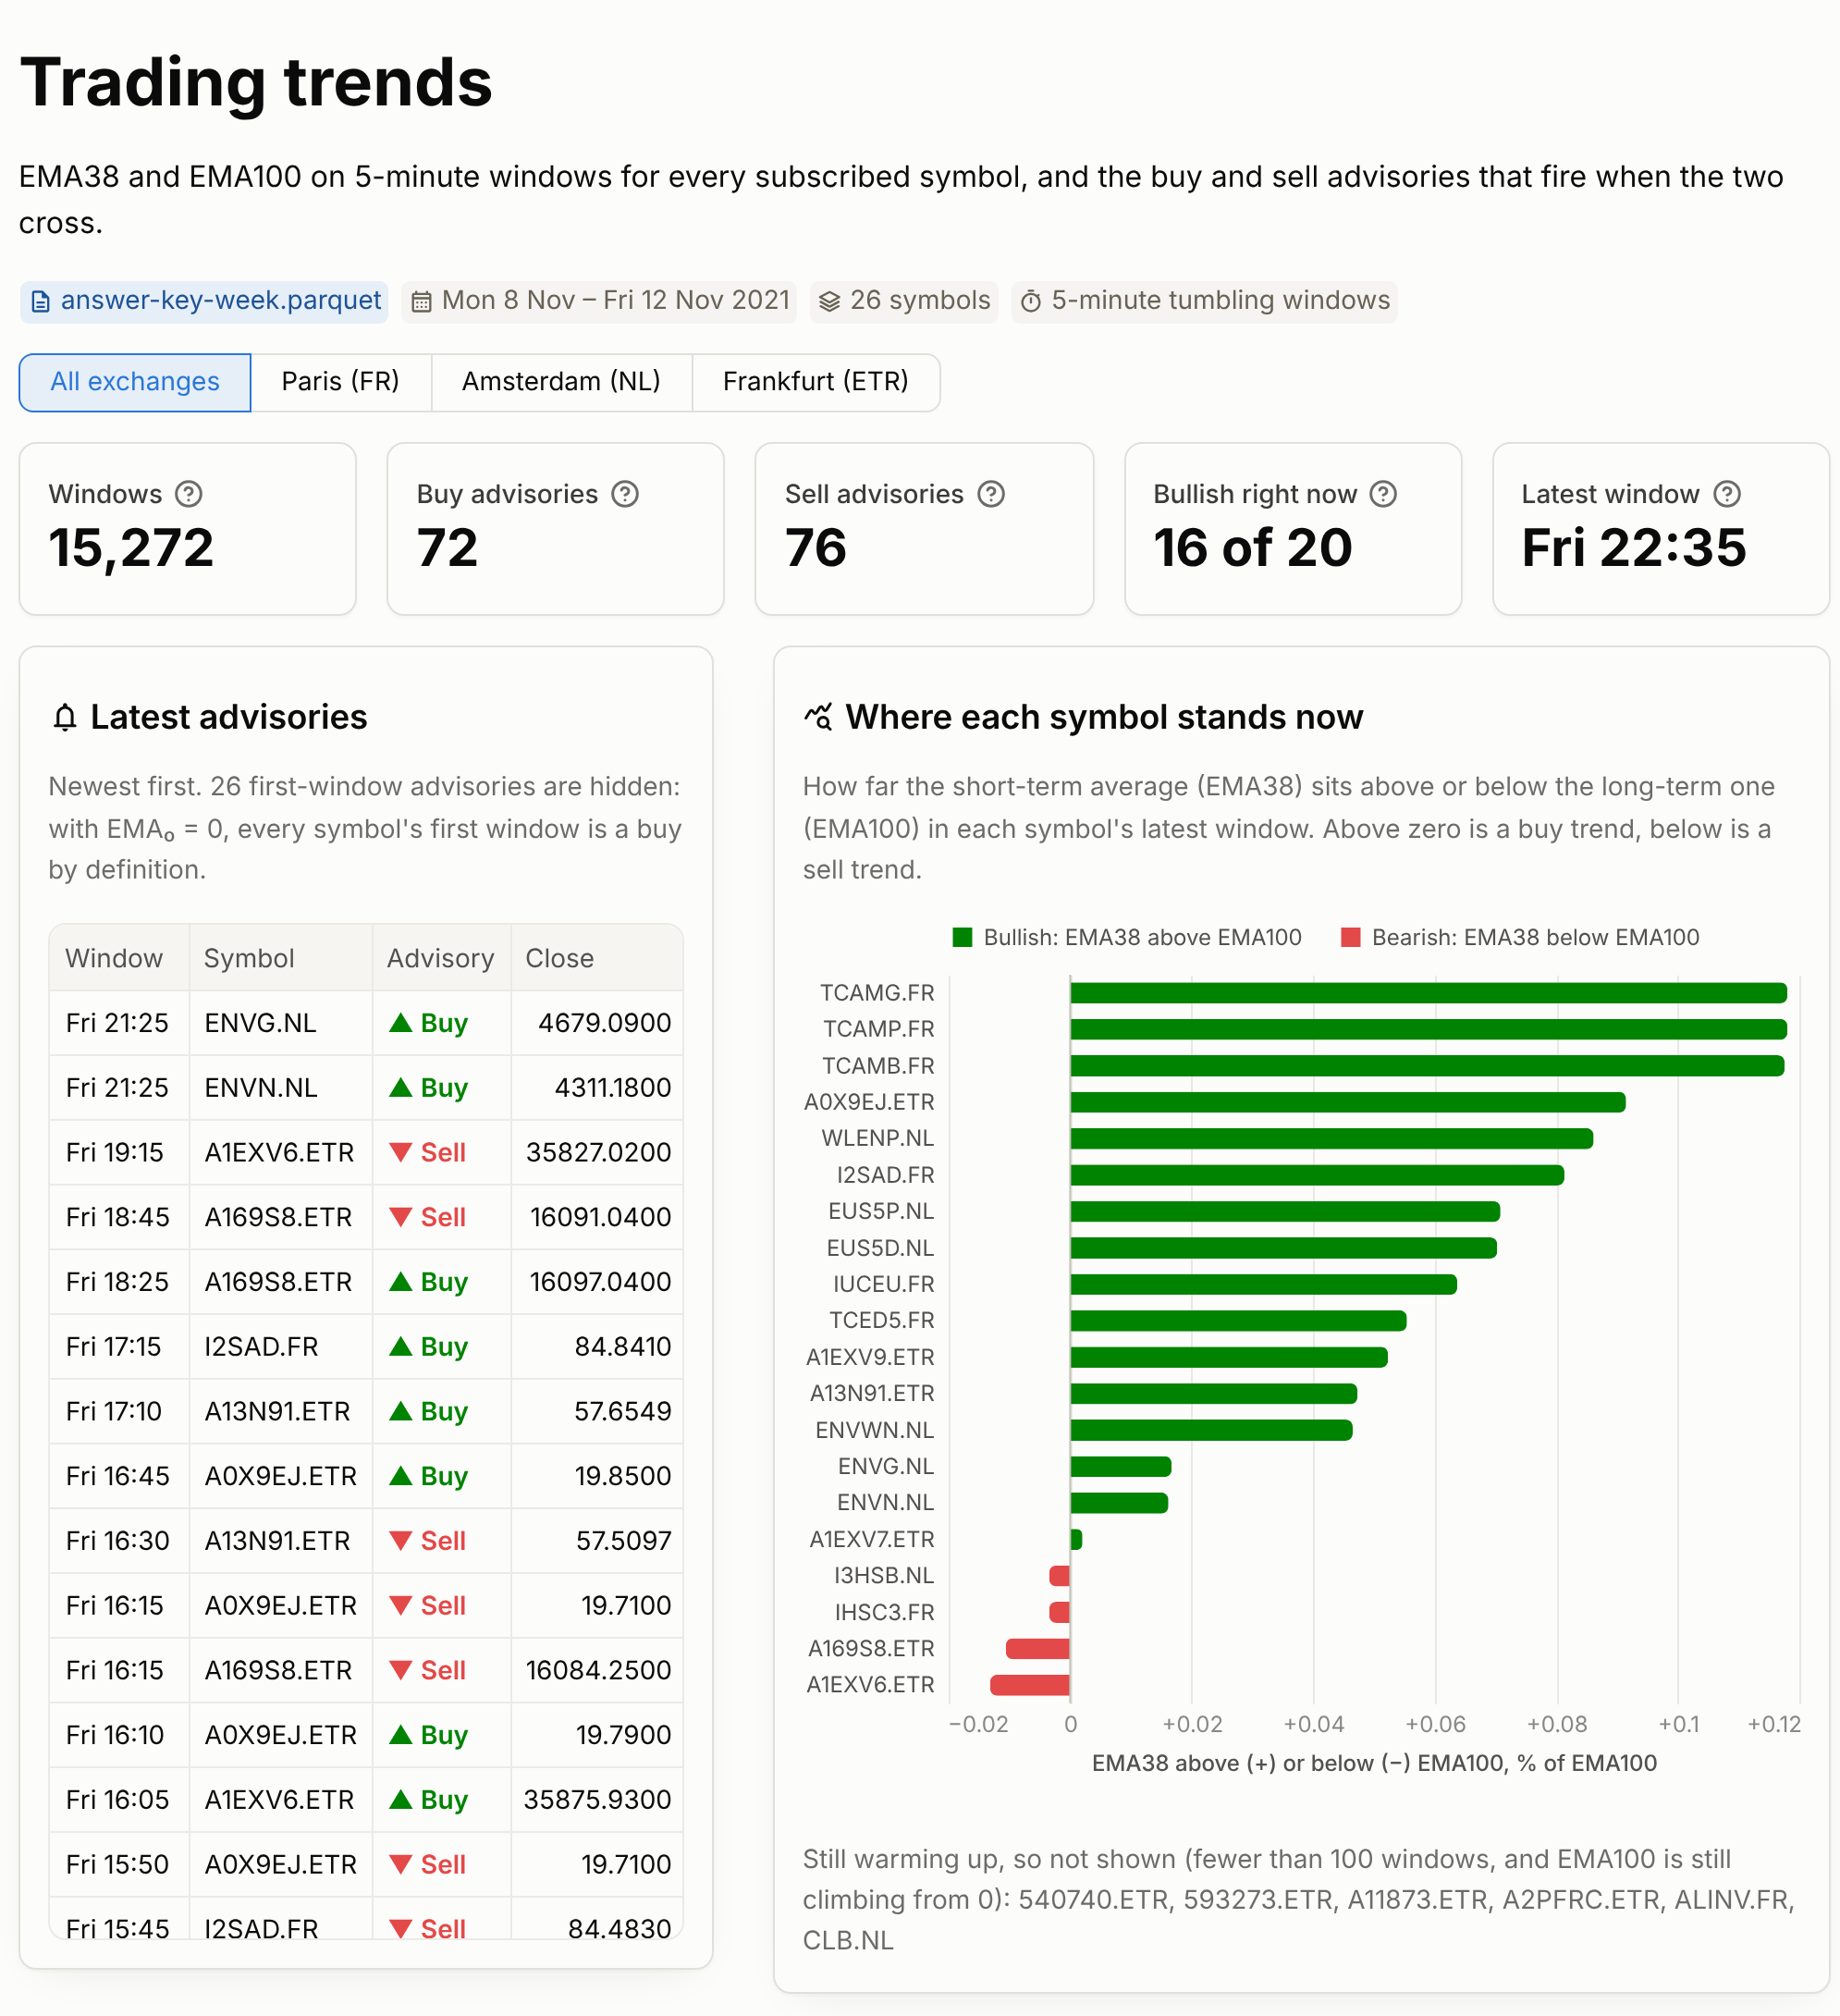
\includegraphics[width=0.8\linewidth]{dashboard-top}
  \caption{Top of the Streamlit dashboard for the 26 subscribed symbols over Mon 8 to Fri 12 Nov: summary figures, latest advisories, and each symbol's EMA38 distance from EMA100 in its latest window.}
  \Description{Dashboard screenshot with five summary tiles (15,272 windows, 72 buy and 76 sell advisories, 16 of 20 symbols bullish, latest window Friday 22:35), a table of the latest buy and sell advisories, and a horizontal bar chart of EMA38 above or below EMA100 per symbol.}
  \label{fig:dashboard}
\end{figure}

%% FACT SHEET: visualization (the rubric has "smart visualization"). Optional extra
%% sentence or two on WHY it is designed this way. Facts:
%%  - First-window advisories hidden by default because with EMA_0 = 0 every symbol's
%%    first window is a buy by definition (26 hidden in the screenshot).
%%  - "Still warming up" list: fewer than 100 windows, EMA100 still climbing from 0.
%%  - The bar chart normalises the EMA gap as % of EMA100 so symbols with prices of 19
%%    and 35,000 can be compared on one axis.
%%  - Exchange tabs; per-symbol chart with "fit to price" so the EMA warm-up from 0 does
%%    not squash the price line; timeline of all advisories shows when markets turned.
%%  - Live Kafka mode or file mode (the same view for the answer key and Flink output).

%% FIXED: removed the Flink UI screenshot ("kafka Flink UI.jpeg"). It was never referenced
%% in the text, its file name had spaces, and it shows the October prototype (Flink 1.20.5,
%% parallelism 1), which no longer matches the system or the experiments below.

%% ---------------------------------------------------------------------------
\section{Performance Evaluation}\label{sec:eval}
%% FIXED: this whole section replaces the draft's evaluation, which described the October
%% prototype: 1,917 test events, one task slot, and a NoResourceAvailableException at
%% parallelism > 1. None of that is true of the current system; every number below comes
%% from results/ in the repository (see results/summary.md and results/RUN-NOTES.md).

\subsection{Experimental setup}
All measurements ran on one laptop, an Apple MacBook Air with an M5 processor (10 cores) and 16\,GB of memory, on mains power. Docker Desktop 29.8.0 was given all 10 cores and 7.75\,GiB of memory. Kafka, the Flink JobManager (1\,GB) and one Flink TaskManager (3\,GB) ran as containers inside it. To test a core count $c$, the TaskManager container was restarted with a CPU limit of $c$ cores and $c$ task slots, and the job was submitted with parallelism $c$. Data: the DEBS 2022 files for Monday 8 to Friday 12 November 2021, checksums verified.
\todo{check the core split of your M5 (performance vs efficiency cores) in System Information and add it here; it matters for the scaling analysis}

\textbf{Scalability method.} The producer first filled the \texttt{ticks} topic with all 59,391,670 weekday trades (183\,s, about 325,000 events/s). For each core count a \emph{bounded} job then read the whole topic and stopped; the processing time is the time between the job's RUNNING and FINISHED states in Flink's REST API, and CPU use was sampled with \texttt{docker stats}. The producer is idle during the measured runs, so it never competes for CPU. The run on 24 November covered 1, 2, 4, 6 and 8 cores with one repeat each; an earlier run on 17 November covered 1, 2 and 4 cores with three repeats each. The same procedure was repeated with every event type (289 million events, including quotes) and with each exchange on its own, at 1, 2 and 4 cores.

\textbf{Latency method.} Monday's busy morning (08:00--12:00, the first 3 million trades, 96,765 windows) was replayed live at 20,000, 50,000 and 100,000 events/s and as fast as possible, against a running job with 4 cores. A window is complete once the first event of the next window has been sent~\cite{frischbier2022gc}; the producer logs that wall-clock moment for every window boundary, and Flink stamps each result with the moment it was produced. Latency is the difference, split into \emph{wait} (until the window fired) and \emph{processing} (after that). Three configurations were measured: the default (5\,s out-of-order bound, Flink's default 100\,ms network buffer timeout and 200\,ms watermark interval), a tuned one (5\,ms buffer timeout, 50\,ms watermark interval) and one with an out-of-order bound of 0.

\subsection{Correctness}
%% FIXED: the draft quoted A169S8.ETR (EMA38 821.9287, EMA100 317.3784) as matching "the
%% expected reference output". That value is real, but it is that symbol's FIRST window
%% (Mon 08:00), whose buy advisory comes from EMA_0 = 0, so it is a weak example. The full
%% comparison below is much stronger evidence.
The output of every Kafka run was compared with the pandas reference, window by window. Table~\ref{tab:correct} shows the result for the full working week; the per-exchange runs, the all-events run and every out-of-order bound on real data passed the same check. The largest relative difference in an EMA value is $8.6\times10^{-12}$, which is floating-point rounding. Of the 11,349 advisories, 4,970 are the first-window buys described in Section~\ref{sec:impl}; the remaining 6,379 also all match. The Docker demo performs the same check automatically on a slice of the real data.

\begin{table}[t]
  \caption{Flink output for Mon--Fri compared with the reference (all exchanges, 8 cores).}
  \label{tab:correct}
  \small
  \begin{tabular}{lrr}
    \toprule
    & Reference & Flink matches\\
    \midrule
    Windows (symbol $\times$ 5 min) & 1,855,645 & 1,855,645\\
    Symbols                         &     4,970 &     4,970\\
    Windows with a value mismatch   &        -- &         0\\
    Advisories (all)                &    11,349 &    11,349\\
    Advisories (not first window)   &     6,379 &     6,379\\
    Missed / spurious / wrong direction & -- & 0 / 0 / 0\\
    \bottomrule
  \end{tabular}
\end{table}

\subsection{Throughput and scalability}
Table~\ref{tab:scal} and Figure~\ref{fig:scal} show the processing time for the 59.4 million weekday trades. It falls from 68.6\,s on one core to 24.1\,s on four and 14.5\,s on eight, a speedup of 4.7. The three-repeat run on 17 November gives the spread: $68.6\pm3.1$\,s, $42.5\pm0.6$\,s and $25.5\pm0.7$\,s for 1, 2 and 4 cores. Table~\ref{tab:scal2} shows the same measurement for every event type and for each exchange.

\begin{table}[t]
  \caption{Weekday trades (59.4 M events), 24 Nov run. Efficiency = speedup / cores; CPU = TaskManager CPU per core.}
  \label{tab:scal}
  \small
  \begin{tabular}{rrrrrr}
    \toprule
    Cores & Time (s) & M events/s & Speedup & Effic. & CPU/core\\
    \midrule
    1 & 68.6 & 0.87 & 1.00 & 1.00 & 93\%\\
    2 & 42.6 & 1.39 & 1.61 & 0.80 & 94\%\\
    4 & 24.1 & 2.47 & 2.85 & 0.71 & 89\%\\
    6 & 20.3 & 2.92 & 3.37 & 0.56 & 79\%\\
    8 & 14.5 & 4.08 & 4.71 & 0.59 & 76\%\\
    \bottomrule
  \end{tabular}
\end{table}

\begin{table}[t]
  \caption{Speedup at 2 and 4 cores for other inputs (24 Nov run; time in seconds at 1 core).}
  \label{tab:scal2}
  \small
  \begin{tabular}{lrrrr}
    \toprule
    Input & Events & 1 core & $2\times$ & $4\times$\\
    \midrule
    All event types & 289.1 M & 147.5 s & 1.70 & 2.66\\
    Trades, FR      &  21.4 M &  31.8 s & 1.63 & 2.81\\
    Trades, ETR     &  32.0 M &  39.0 s & 1.76 & 2.82\\
    Trades, NL      &   6.0 M &  13.2 s & 1.44 & 2.64\\
    \bottomrule
  \end{tabular}
\end{table}

\begin{figure}[t]
  \centering
  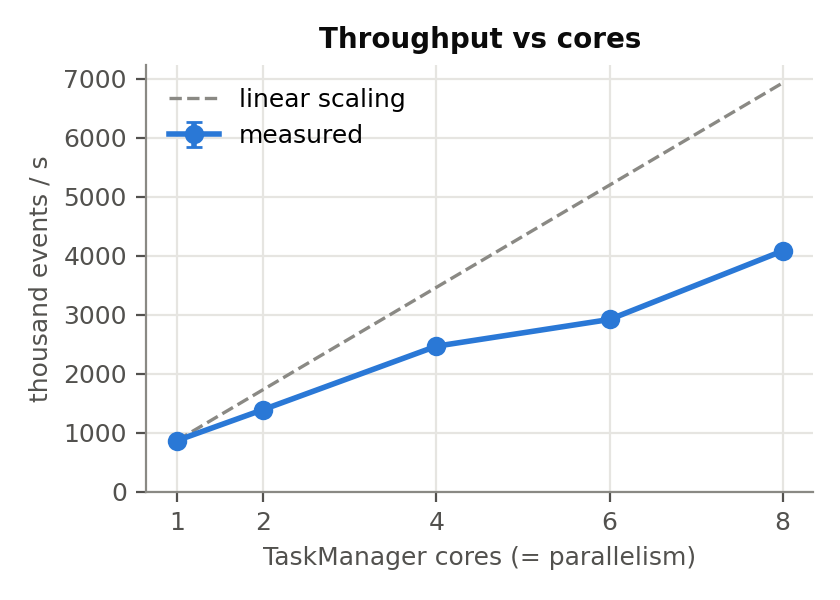
\includegraphics[width=0.75\linewidth]{scalability-throughput}
  \caption{Throughput for the weekday trades against TaskManager cores (= parallelism), with linear scaling from the 1-core result for comparison.}
  \Description{Line chart: measured throughput rises from about 0.87 million events per second at 1 core to 4.08 million at 8 cores, below a dashed linear-scaling line that reaches about 6.9 million.}
  \label{fig:scal}
\end{figure}

%% FACT SHEET: scalability analysis (the course explicitly asks you to "explain the observed
%% results, including any limitations or lack of speedup"). What we observed:
%%  - Speedup 1.61 / 2.85 / 3.37 / 4.71 at 2 / 4 / 6 / 8 cores; efficiency drops from
%%    0.80 to 0.56-0.59. Throughput 0.87 -> 4.08 M events/s.
%%  - 6 cores is the weak point: 4 -> 6 cores gains only 18% (24.1 -> 20.3 s), while
%%    6 -> 8 gains 40% (20.3 -> 14.5 s).
%%  - CPU per core stays high up to 4 cores (89-94%) and then drops (79% at 6, 76% at 8):
%%    the extra cores are not fully busy.
%%  - The all-events input scales a bit worse at 4 cores (2.66) than trades only (2.85),
%%    although it has 4.9x the events but the same windows.
%%  - NL (smallest input, 6.0 M events, 13 s) scales worst at 2 cores (1.44) and its
%%    CPU/core at 4 cores is only 42%.
%% Candidate explanations to weigh (say which the evidence supports, and how sure you are):
%%  a) Kafka partitions: the topic has 8 partitions. With 6 source instances, 2 of them
%%     read 2 partitions and 4 read 1, so the slowest source has twice the work -> fits
%%     the 6-core dip and the recovery at 8 (8 partitions / 8 instances = 1 each).
%%     Evidence: the 4->6 vs 6->8 numbers; at 4 cores each instance reads exactly 2.
%%  b) Shared machine: Kafka, the JobManager and Docker itself run on the same 10 cores
%%     as the TaskManager; at 8 TaskManager cores the broker has little left.
%%     Evidence: CPU/core falls at 6 and 8; Docker has 10 CPUs in total.
%%  c) Performance vs efficiency cores on the M5: beyond the number of P-cores, extra
%%     cores are slower ones. (Needs the core split from the TODO above.)
%%  d) Passively cooled MacBook Air: may throttle in longer runs. Evidence is weak: the
%%     1-core run (the longest) has the largest spread, +-3.1 s over 3 repeats.
%%  e) Fixed costs that do not parallelise: job start-up, reading the topic metadata, the
%%     final end-of-stream flush. Their share grows as runs get shorter (NL at 4 cores
%%     runs only 5 s) -> fits NL's poor efficiency.
%%  f) Network shuffle: two keyBy steps mean every record crosses instances twice
%%     (hash partitioning). With 1 instance that traffic is local.
%%  g) Quotes are dropped right after the source, so for the all-events run the extra
%%     work is parsing; parsing scales with source instances (again partitions).
%% Limitations to state: one repeat per point on 24 Nov (the 17 Nov repeats give the
%% spread), a single TaskManager, a laptop, and everything sharing one Docker VM.
\todo{scalability analysis paragraph, see the fact sheet}

\subsection{Latency}
Table~\ref{tab:lat} shows the latency at 4 cores. In every configuration almost all of it is wait time: the median processing time after a window fires is 2 to 4\,ms, and its 99th percentile 34 to 229\,ms. With the tuned settings the median falls from 266\,ms to 93\,ms at 100,000 events/s. The maximum rate reached by the producer was about 290,000--313,000 events/s.

\begin{table}[t]
  \caption{Latency in ms from window completion to EMA result, 4 cores, 96,765 windows per run. ``max'' = producer at full speed (about 290k--313k events/s).}
  \label{tab:lat}
  \small
  \begin{tabular}{lrrrrr}
    \toprule
    Config. & Rate (ev/s) & p50 & p95 & p99 & wait p50\\
    \midrule
    Default    &  20k & 408 & 524 & 621 & 385\\
               &  50k & 276 & 398 & 464 & 261\\
               & 100k & 266 & 400 & 557 & 239\\
               &  max & 206 & 490 & 516 & 198\\
    \midrule
    Tuned      &  20k & 256 & 285 & 464 & 253\\
               &  50k & 140 & 170 & 370 & 137\\
               & 100k &  93 & 191 & 381 &  89\\
               &  max &  80 & 521 & 546 &  77\\
    \midrule
    OOO = 0    &  20k & 237 & 352 & 422 & 224\\
               &  50k & 230 & 327 & 364 & 223\\
               & 100k & 232 & 308 & 369 & 222\\
               &  max & 252 & 466 & 478 & 239\\
    \bottomrule
  \end{tabular}
\end{table}

%% Dropped the latency figure to stay within 5 pages; Table 5 has the same numbers.
%% figures/latency-vs-rate-tuned.png is still here if you prefer the figure over the table.

%% FACT SHEET: latency analysis. What we observed:
%%  - Latency is almost all "wait" (boundary -> window fired); processing after firing
%%    is 2-4 ms median in every run.
%%  - Default config: median latency FALLS as the rate rises (408 -> 276 -> 266 -> 206 ms).
%%    Same with tuned (256 -> 140 -> 93 -> 80 ms). Counter-intuitive: more load, less
%%    latency.
%%  - Tails rise at full speed: tuned p95 jumps from 191 to 521 ms and p99 to 546 ms;
%%    processing p99 rises to 229 ms. Default p95 at max is 490 ms.
%%  - Tuning (5 ms buffer timeout, 50 ms watermark interval) cuts the median by
%%    about 1.6x-3x at 20k-100k ev/s; at max the tails are no better.
%%  - OOO = 0 run (24 Nov, default knobs) is flat at ~230 ms median whatever the rate.
%%    Careful comparing it with "default": different day (17 vs 24 Nov), so a 5 s bound
%%    vs 0 s is not the only difference.
%% Candidate explanations to weigh:
%%  a) Why wait dominates: a window can only fire when the watermark passes its end, and
%%     the watermark needs (i) the slowest of the 8 partitions to move past it,
%%     (ii) the out-of-order allowance, measured in EVENT time, and (iii) the periodic
%%     watermark emission (200 ms default, 50 ms tuned).
%%  b) Why more load means less latency: the 5 s out-of-order bound is event time. At a
%%     higher replay rate, 5 s of market time passes in less wall-clock time, so the
%%     watermark catches up sooner. Also network buffers (100 ms default timeout) fill and
%%     flush sooner when more data flows. Check: is the effect smaller for OOO = 0, where
%%     the bound is not in play? (It is: flat ~230 ms.)
%%  c) Why tuning helps most at moderate rates: the buffer timeout and watermark interval
%%     are fixed wall-clock delays that dominate when data is sparse.
%%  d) Why tails grow at max rate: the system starts queueing (source or Kafka broker on
%%     the same machine, 4 TaskManager cores out of 10 shared), processing p99 rises.
%%  e) The OOO = 0 puzzle: you would expect it to be lowest everywhere, but at 50k-100k
%%     the tuned 5 s run is lower. That suggests the knobs (buffer timeout / watermark
%%     interval) matter more than the bound once the rate is high. Worth saying honestly.
%% Relate it to the requirement: an advisory within ~0.1-0.6 s of the window completing,
%% for 5-minute windows.
\todo{latency analysis paragraph, see the fact sheet}

\subsection{Long-tail distribution and load balance}
Although the event counts per symbol span five orders of magnitude (Figure~\ref{fig:longtail}), the window operator's load is close to even: at 8 cores the busiest instance received 8.52 million records against a mean of 7.42 million, a max/mean ratio of 1.15 (1.00 is perfectly even). At 4 cores the ratio is 1.05 for Paris, 1.07 for Amsterdam, 1.14 for Frankfurt and 1.10 with every event type.

%% FACT SHEET: long tail. Observed: max/mean 1.15 at 8 cores (instances got 6.39 M to
%% 8.52 M records), 1.05-1.14 at 4 cores. Rare symbols cost almost nothing (state is two
%% doubles per symbol; windows without trades never fire).
%% Explanations to weigh:
%%  - With ~5,000 keys hashed onto 4-8 instances, the many mid-size symbols average out;
%%    the busiest symbol has at most ~32k trades/day, small next to 59 M.
%%  - The trade distribution is flatter than the event distribution (Section 2), and only
%%    trades reach the keyed operators, so the extreme skew of the raw events never
%%    reaches the windows.
%%  - Remaining imbalance (1.15): hash collisions of a few busy symbols on one instance.
%%  - What would break it: one symbol bigger than 1/parallelism of all trades. Not the
%%    case here; mention key-splitting / two-stage aggregation as the fix if it were.
%%  - Long tail in time, too: the warm-up of rare symbols (1,263 symbols with < 38
%%    windows), handled in the dashboard.
\todo{long-tail paragraph, see the fact sheet}

\subsection{Design trade-off: out-of-order bound}
On the real Monday no trade arrives after its window has been passed, so every bound from 0 to 120\,s gives exactly the reference output (0 late trades, all 4,840 expected advisories correct). To show what the bound buys, we generated 3 million events in the same layout in which 2\% of the trades arrive up to 60\,s late, and ran the job with bounds from 0 to 120\,s (file mode, parallelism 4, on a 4-core x86-64 Linux cloud container). Table~\ref{tab:ooo} shows the result.

\begin{table}[t]
  \caption{Synthetic input with 2\% of trades up to 60\,s late: late trades set aside and windows that differ from the reference, per out-of-order bound.}
  \label{tab:ooo}
  \small
  \begin{tabular}{rrrr}
    \toprule
    Bound (s) & Late trades & Wrong windows & Wrong advisories\\
    \midrule
    0   & 14 & 517 & 4\\
    1   &  2 & 229 & 2\\
    5   &  5 & 114 & 1\\
    15  &  2 & 114 & 1\\
    30  &  0 &   0 & 0\\
    60  &  0 &   0 & 0\\
    120 &  0 &   0 & 0\\
    \bottomrule
  \end{tabular}
\end{table}

%% FACT SHEET: out-of-order bound. Observed: on synthetic data, wrong windows fall from 517
%% (bound 0) to 0 from 30 s up; run time stays about 11 s at every bound (10.5-12.0 s), so
%% a bigger bound costs no throughput, only latency (it delays every window by up to the
%% bound in event time). Real Monday: no disorder at all, any bound is correct.
%% Oddities to explain or mention: "late trades" is not monotonic (14, 2, 5, 2) while
%% wrong windows are; one late trade can make many windows wrong because the EMA carries
%% the error into every later window of that symbol. 30 s suffices although trades are up
%% to 60 s late: a trade is only late if the watermark has passed its window's END, and
%% most delayed trades still fall in a window that is open.
%% Your choice to justify: default 5 s (what it costs in latency vs what it protects).
\todo{trade-off paragraph and why you chose 5\,s, see the fact sheet}

%% ---------------------------------------------------------------------------
\section{Conclusion}\label{sec:concl}
%% FACT SHEET: conclusion. Your draft's conclusion is kept below in a comment; it is fine
%% as a summary but misses the results. Facts you may want to pull in:
%%  - Exact match with the reference on 1,855,645 windows and 11,349 advisories.
%%  - 0.87 -> 4.08 M events/s from 1 to 8 cores (4.7x), with the limits you identified.
%%  - Median latency 80-408 ms depending on rate and settings; nearly all of it is
%%    waiting for the watermark, not processing.
%%  - Long tail handled: load max/mean 1.15 at 8 cores.
%% Limitations / future work candidates: single laptop and single broker; one repeat per
%% point in the 1-8 core run; checkpointing off; multiple TaskManagers / a real cluster;
%% more Kafka partitions than 8; per-symbol latency for rare symbols.
%%
%% Your draft text, for reference:
%% This project implemented a real-time financial tick data processing pipeline using Apache
%% Kafka and Apache Flink. The system successfully processed streaming trade events,
%% calculated EMA38 and EMA100 values, detected bullish and bearish trading signals and
%% published results to an output Kafka topic. A Streamlit dashboard was developed to
%% visualize EMA trends and signal events. Validation against the provided reference dataset
%% confirmed the correctness of the implementation. The project demonstrates the use of
%% distributed stream processing techniques for real-time financial market analysis.
\todo{conclusion, see the fact sheet}

%% ---------------------------------------------------------------------------
\section{Individual Contributions}\label{sec:contrib}

%% Each member answers the same three questions, in their own words.
%% Be specific about what you personally did, and be honest about the team.

\subsection{\texorpdfstring{{Yashasvi Mishra}}{Yashasvi Mishra}}
\begin{enumerate}
  \item \textbf{Most important design decisions.} The most important design decision was to implement the processing logic using Apache Flink event-time semantics instead of processing-time semantics. This allowed financial trade events to be processed according to their actual trade timestamps and enabled correct handling of windowed aggregations. Another key decision was to use keyed state for incremental EMA38 and EMA100 calculations, which avoided repeated processing of historical data and allowed efficient real-time computation.
  \item \textbf{Most challenging parts.} The most challenging part of the project was implementing and validating the EMA computation pipeline. Correct handling of timestamps, watermarks, five-minute tumbling windows and stateful EMA calculations required extensive testing and debugging. Integration between Flink, Kafka and the output Kafka sink also presented challenges, particularly when serializing output records and debugging runtime configuration issues.
  \item \textbf{Your contribution and the team's functionality.} My primary contribution focused on implementing the Apache Flink processing pipeline. This included trade event processing, timestamp assignment, watermark handling, tumbling event-time windows, EMA38 and EMA100 computation, buy and sell signal detection and publication of processed results to the \texttt{ema-results} Kafka topic. I also developed the Streamlit dashboard used to visualize EMA values, trading signals and summary statistics. In addition, I participated in system integration, validation against the provided reference output and preparation of the final project report.
\end{enumerate}
%% Note for Yashasvi (not changed, her words): "the provided reference output" was our own
%% pandas answer key, not something the course provided; she may want to adjust that.

\subsection{\texorpdfstring{{Manas Vernekar}}{Manas Vernekar}}
%% FACT SHEET: your contribution. From the project records; keep only what is true and
%% add what is missing, in your own words:
%%  - Data exploration in pandas: the long-tail analysis and figure, the two clocks,
%%    late and placeholder trades (analysis/ folder).
%%  - The pandas answer key for the full week (EMAs and crossovers), which every
%%    correctness claim in this report rests on.
%%  - November rework with an AI coding agent (PRs #2-#4): Flink job rewrite (event
%%    classification, per-partition watermarks, tie-break, subscriptions, late side
%%    output), producer rewrite, validator, Docker images and Compose setup, experiment
%%    scripts, rebuilt dashboard. You reviewed and merged these and need to be able to
%%    explain them.
%%  - Ran all experiments on your MacBook (17 and 24 Nov), including the 1-8 core run.
%%  Questions to answer: which design decision mattered most to you? What was hardest
%%  (e.g. the Kafka retention bug that deleted 2021-stamped output, idle-partition late
%%  trades fixed by the start marker, scaling past one task slot)? How did the team work?
\begin{enumerate}
  \item \textbf{Most important design decisions.} \todo{your answer}
  \item \textbf{Most challenging parts.} \todo{your answer}
  \item \textbf{Your contribution and the team's functionality.} \todo{your answer}
\end{enumerate}

%% ---------------------------------------------------------------------------
%% The course asks for a brief disclosure of how AI tools were used in the
%% project and the report. Be honest and specific here.
\section*{Use of AI Tools}
%% FACT SHEET: what the disclosure has to cover so it matches what actually happened.
%% Your draft text is below; it currently understates the code and report help.
%%  - Code: Claude Code wrote most of the November rework (PRs #2-#4: Flink job, producer,
%%    validator, Docker, experiments, dashboard). Say that, and how you verified it
%%    (reviewed the PRs, re-ran validation and experiments yourselves).
%%  - Report: Claude fixed LaTeX and factual errors, wrote the setup, method and results
%%    descriptions, tables, captions and the architecture figure from the results/ data,
%%    and prepared fact sheets; you wrote the analysis, interpretation and conclusions.
%%    You said the teacher allowed this; say so explicitly, since the written course
%%    rules only allow proofreading for the report.
%%  - Copilot use, if any, as in your draft.
%%
%% Draft text: Microsoft Copilot and Claude were used as auxiliary tools during the project.
%% AI assistance was primarily used for explaining Apache Flink concepts, debugging build
%% and configuration issues, reviewing code snippets, suggesting dashboard improvements and
%% providing feedback on report structure. All implementation decisions, system integration,
%% validation of results, performance evaluation and final report content were reviewed and
%% verified by the authors. AI-generated suggestions were adapted where necessary to fit the
%% project requirements and the implemented system.
\todo{AI-use disclosure, see the fact sheet}

%% ---------------------------------------------------------------------------
\bibliographystyle{ACM-Reference-Format}
\bibliography{references}

\end{document}
